\documentclass[aspectratio=1610]{beamer}
\usepackage[utf8]{inputenc}
\usepackage{polski}
\usepackage[T1]{fontenc}
\usepackage{tikz}
\usepackage{tikzducks}
% \usetikzlibrary{decorations.pathmorphing}
\usepackage{multimedia}
\usepackage{graphicx}
\usepackage[justification=centering]{caption}
\usepackage{textcomp}
\usepackage{appendixnumberbeamer}
\usepackage{qrcode}
% \usepackage[natbib, language=polish, sorting=none]{biblatex}
% \addbibresource{lio.bib}
\usepackage{hyperref}
%\usepackage[width=\textwidth]{animate}
%\usepackage{chemformula}
\usepackage{sidecap}
\usepackage{multirow}
\usepackage{multicol}
\usepackage{rotating}
\usepackage{anyfontsize} % change font size for semposiwko

\usepackage{physics}
\usepackage{array}
\usepackage{booktabs}
\usepackage{transparent}
% \usepackage{siunitx}
% \usepackage[rightcaption]{sidecap}
\usepackage{eso-pic}

\usepackage{listings}
\lstset{
basicstyle=\small\ttfamily,
columns=flexible,
breaklines=true
}

% \usepackage{emoji}
\usepackage{subcaption}


\usepackage[natbib, sorting=none]{biblatex}
\addbibresource{lio.bib}
\renewcommand*{\bibfont}{\scriptsize}

\usefonttheme[onlymath]{serif}

\usetheme{Szeged}
\usecolortheme{whale}
\setbeamercolor{palette primary}{bg=violet!80!black,fg=white}
\setbeamercolor{palette secondary}{bg=violet!60!black,fg=white}
% \definecolor{deepviolet}{RGB}{46,0,79}
% \definecolor{vividpink}{RGB}{255,0,127}
% \setbeamercolor{palette primary}{bg=deepviolet,fg=white}
% \setbeamercolor{palette secondary}{bg=vividpink,fg=white}
\setbeamercolor{palette tertiary}{bg=violet!40!black,fg=white}
\setbeamercolor{palette quaternary}{bg=violet!20!black,fg=white}
\setbeamercolor{structure}{fg=violet!60!black}
\setbeamertemplate{caption}{\insertcaption}
% \setbeamertemplate{headline}{
%   \begin{beamercolorbox}[wd=.9\paperwidth]{headline}
%     \vspace{1.5ex}
%     \insertsectionnavigationhorizontal
%     \vspace{1.5ex}
%   \end{beamercolorbox}
% }
% \definecolor{violet-dark}{HTML}{4B0082}
% \definecolor{teal}{HTML}{008080}
% \definecolor{amber}{HTML}{FFC107}
% \definecolor{light-grey}{HTML}{F5F5F5}
% \definecolor{charcoal}{HTML}{333333}
% \setbeamercolor{palette primary}{bg=violet-dark, fg=white}
% \setbeamercolor{palette secondary}{bg=teal, fg=white}
% \setbeamercolor{palette tertiary}{bg=amber, fg=charcoal}
% \setbeamercolor{background canvas}{bg=light-grey}
% \setbeamercolor{normal text}{fg=charcoal}
% Główna paleta fioletów
% \definecolor{coolblack}{HTML}{000000}
% \definecolor{coolnavy}{HTML}{14213D}
% \definecolor{coolorange}{HTML}{FCA311}
% \definecolor{coollightgray}{HTML}{E5E5E5}
% \definecolor{coolwhite}{HTML}{FFFFFF}

% % Opcjonalnie: ustawienia kolorów dla Beamera
% \setbeamercolor{normal text}{fg=coolblack,bg=coolwhite}
% \setbeamercolor{structure}{fg=coolorange}
% \setbeamercolor{frametitle}{fg=coolwhite,bg=coolnavy}
% \setbeamercolor{title}{fg=coolwhite,bg=coolnavy}
% \setbeamercolor{item}{fg=coolorange}
% \setbeamercolor{block title}{fg=coolwhite,bg=coolnavy}
% \setbeamercolor{block body}{fg=coolblack,bg=coollightgray}
% \setbeamercolor{palette tertiary}{fg=coolwhite, bg=coolorange}
% \setbeamercolor{palette quaternary}{fg=coolblack, bg=coollightgray}

\linespread{0.8}

\setbeamertemplate{background}%
{%
    \begin{tikzpicture}[remember picture,overlay]{\node[yshift=1.5cm,xshift=-2cm,opacity=0.1] at (current page.south east)
      {
      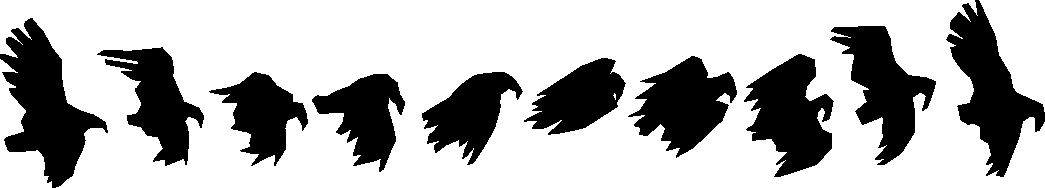
\includegraphics[scale=0.4, angle=25]{ptaki.pdf}
      }
      ;
    \node[yshift=-2cm,xshift=-2cm,opacity=0.05] at (current page.north east)
      {
      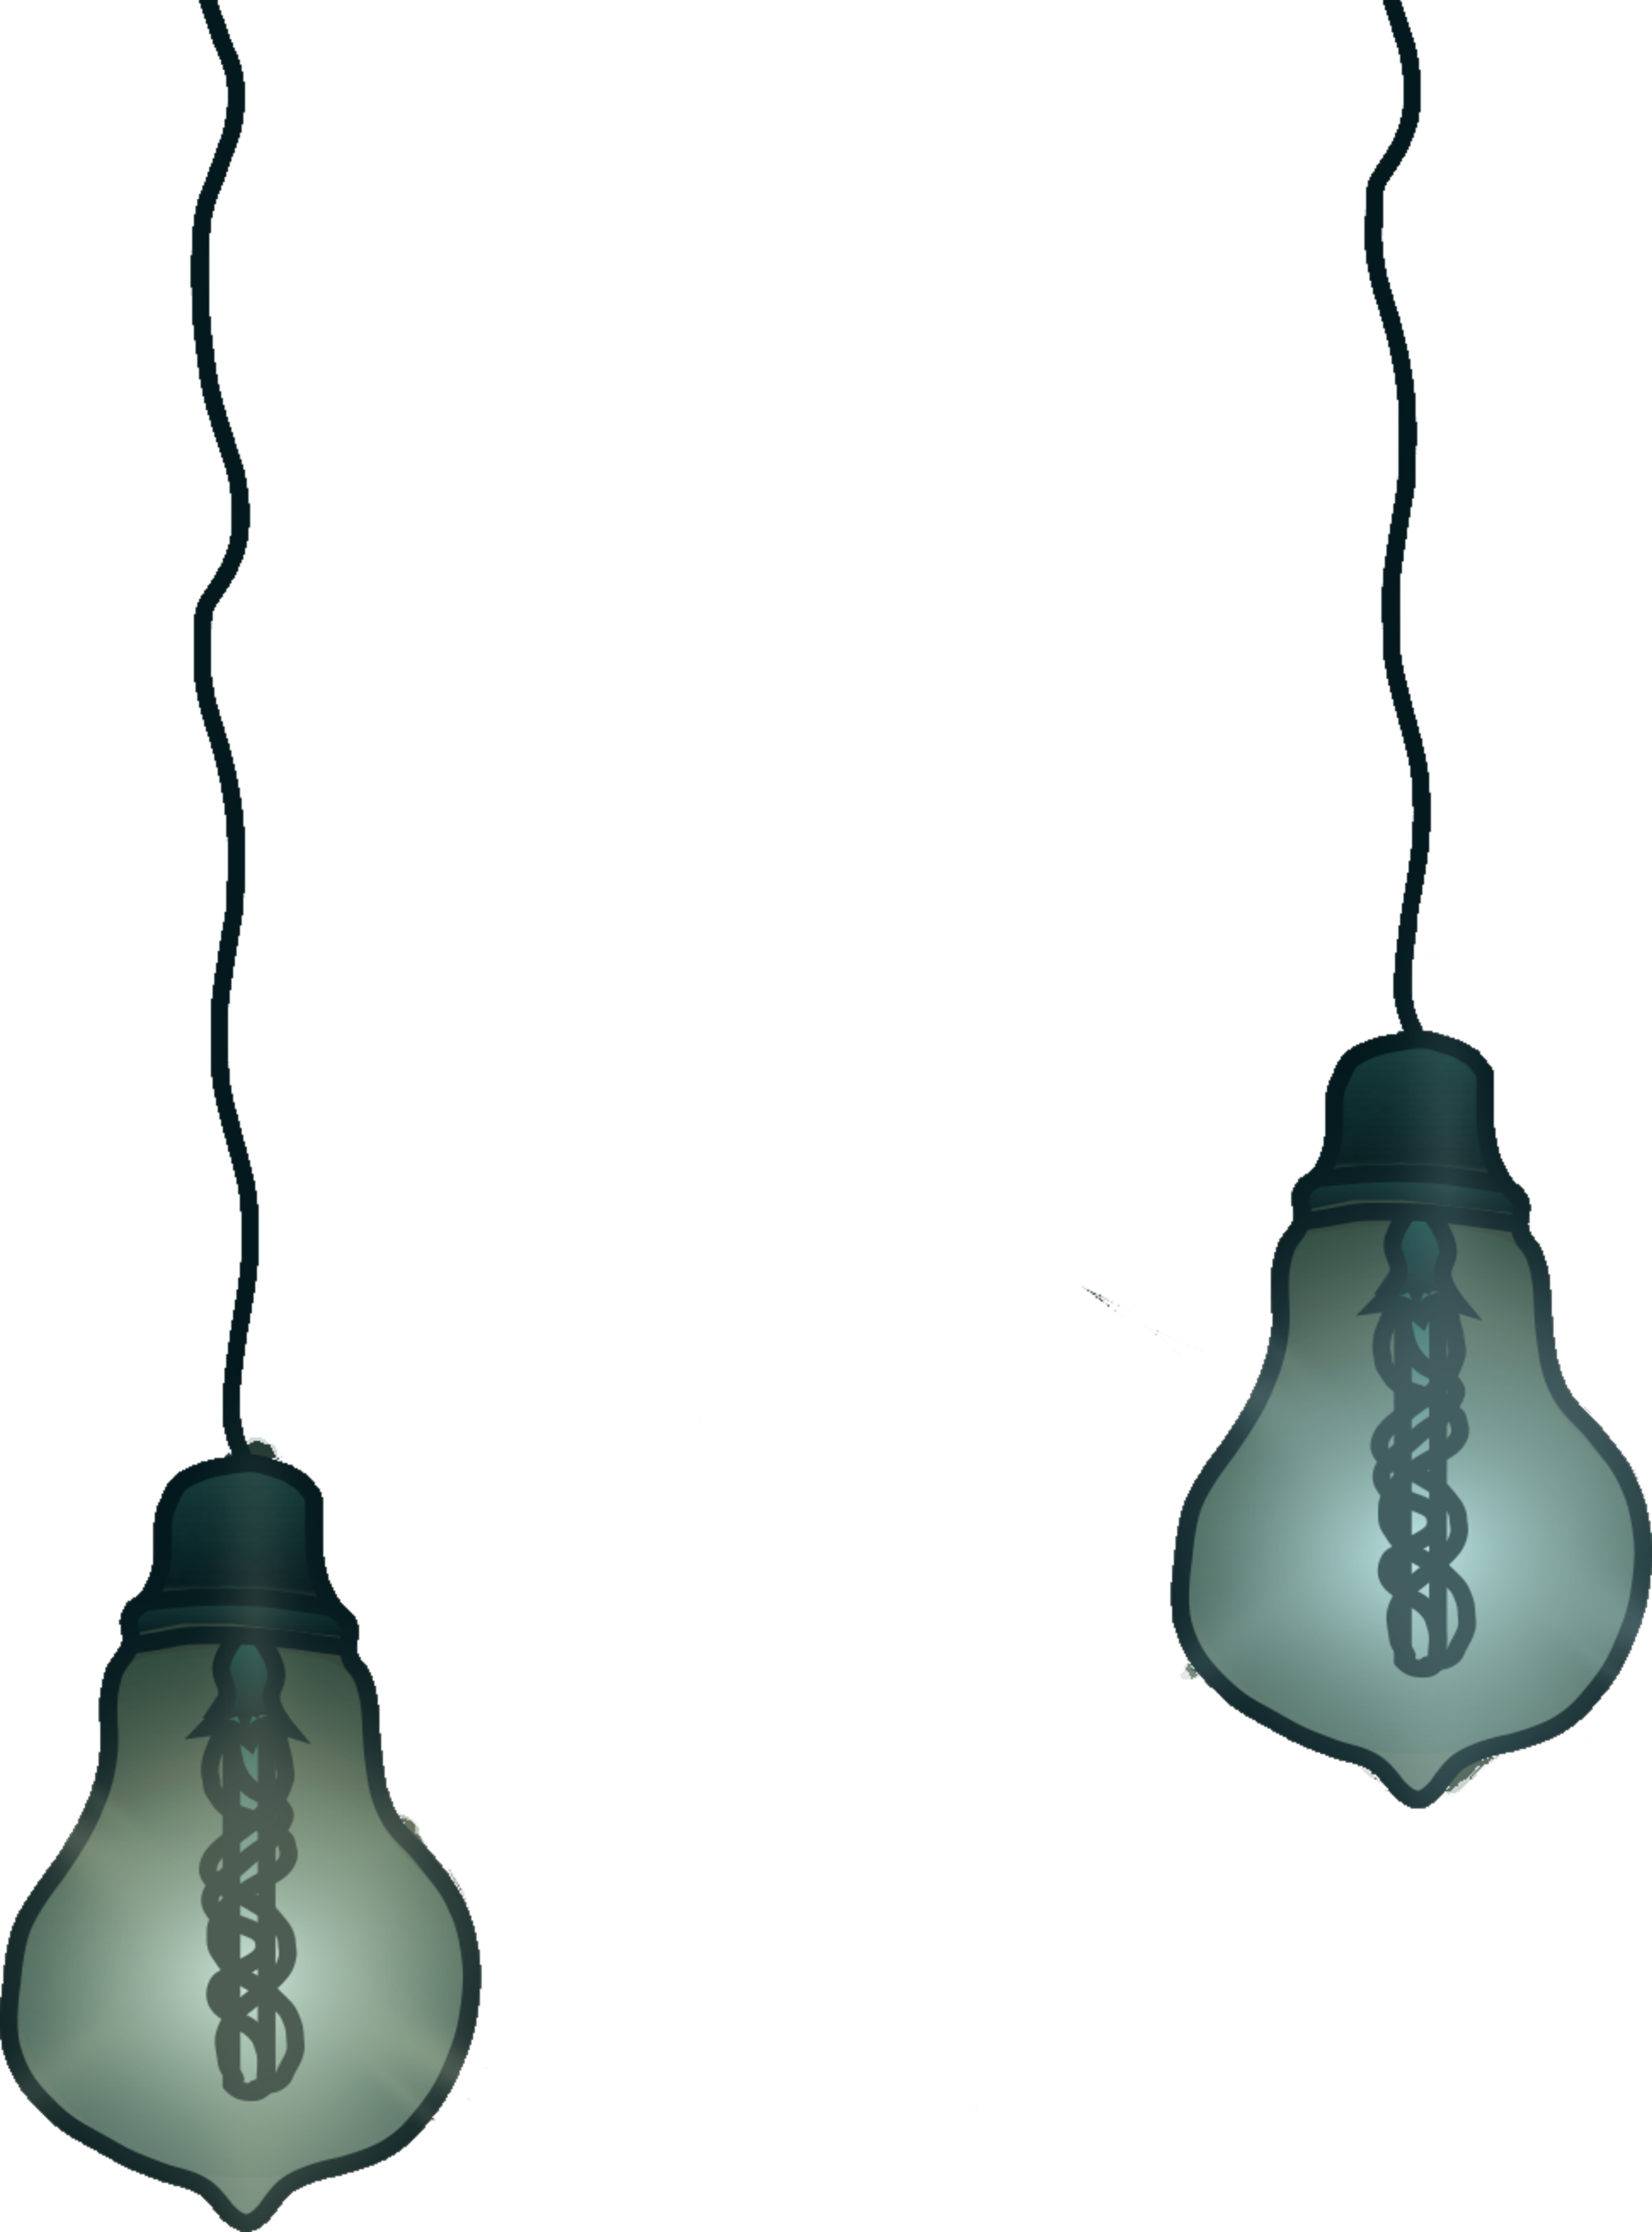
\includegraphics[scale=0.1, angle=0]{zarowki.pdf}
      }
      ;
    \node[yshift=1.0cm,xshift=0.6cm] (logopos) at (current page.south west) {{\begin{tikzpicture}\shuffleducks\duck[signpost=\insertframenumber, \randomhead,scale=.4]\end{tikzpicture}}};
    \pgfmathsetmacro{\progress}{360*(\insertframenumber)/(\inserttotalframenumber)};
    \draw[line width=0.2*3pt] ([xshift=0.55cm] logopos)  arc[radius=0.55cm, start angle=0, end angle=\progress];
    \fill ([shift={(\progress:0.55cm)}] logopos) circle(1pt);

    }
        \end{tikzpicture}
    
}

\newcommand{\SeMPowisko}{%
\large S\normalsize%
\kern-.3em \lower.2ex\hbox{e}%
\lower.2ex\hbox{\large M\normalsize}%
\kern-.1em \raise.1ex\hbox{\large P\normalsize}%
\kern-.3em \lower.2ex\hbox{o}%
\kern-.2em \raise.2ex\hbox{w}%
\lower.2ex\hbox{i}%
s%
\raise.2ex\hbox{k}%
\kern-.3em \lower.2ex\hbox{o}%
}
% \usepackage{microtype}
% \DeclareRobustCommand{\SeMPowisko}{SeMPowisko}


% \newcommand\Tikz{Ti\emph{k}Z}
% \definecolor{neworange}{RGB}{255,140,0}
% \renewcommand{\figurename}{figure}


\title{Efekt hydrofobowy}
\subtitle{za: Charles Tanford „The hydrophobic effect: formation of micelles”}
% \subtitle{Building a Low-Cost Ground Station with SatNOGS}
\author[M. Winiarski]{Mateusz ,,\(\blacksquare\)'' Winiarski}
\institute[Seminarium magisterskie]{biofizyka, FAIS, Uniwersytet Jagielloński}
\date[dzisiaj]{dzisiaj}

\begin{document}

\frame{\titlepage}

\nocite{Tanford_1980}

\begin{frame}{}{}
  \flushright
  \emph{The antipathy of the paraffin-chain for water is, however, frequently misunderstood. There is no question of actual repulsion between individual water molecules and paraffin chains, nor is there any very strong attraction of paraffin chains for one another. There is, however, a very strong attraction of water molecules for one another in comparison with which the paraffin-paraffin or paraffin-water attractions are very slight.}
  \\[5mm]
  \emph{(Antypatia łańcucha parafinowego do wody jest jednak często źle rozumiana. Nie ma mowy o rzeczywistym odpychaniu pomiędzy poszczególnymi cząsteczkami wody i łańcuchami parafinowymi, ani nie istnieje bardzo silne przyciąganie się łańcuchów parafinowych do siebie. Istnieje jednak bardzo silne przyciąganie się cząsteczek wody do siebie, w porównaniu z którym przyciąganie parafina-parafina lub parafina-woda jest bardzo niewielkie.)}
\\[5mm]
  G. S. Hartley (1936) 
\end{frame}

% \begin{frame}
%   W swej istocie efekt hydrofobowy wynika z tego, że substancje niepolarne, takie jak węglowodory (węglowodory alifatyczne są najbardziej zbliżone do czysto hydrofobowego charakteru) i gazy obojętne, wykazują minimalną rozpuszczalność w wodzie. Gdy cząsteczki hydrofobowe są obecne w wodzie, woda w ich otoczeniu tworzy uporządkowane struktury klatkowe (klatraty), co prowadzi do zmniejszenia entropii (wzrostu uporządkowania) układu. Ten niekorzystny termodynamicznie spadek entropii jest dominującym czynnikiem napędzającym efekt hydrofobowy. W konsekwencji, substancje hydrofobowe mają tendencję do minimalizowania kontaktu z wodą poprzez agregację, co jest podstawą do tworzenia micel (gdzie hydrofobowe ogony gromadzą się w centrum, a polarne głowy są na zewnątrz) oraz dwuwarstw lipidowych, które tworzą błony biologiczne. Efekt hydrofobowy jest również kluczowy dla zwijania się białek (protein folding), gdzie hydrofobowe łańcuchy boczne aminokwasów są często ukrywane we wnętrzu białka, aby unikać kontaktu z wodą.
% \end{frame}

% \begin{frame}
%   Struktura wody: Woda jest cieczą o bardzo uporządkowanej strukturze. Cząsteczki wody tworzą rozległą sieć powiązań wodorowych, gdzie każda cząsteczka H2O może tworzyć cztery wiązania wodorowe, przyjmując tetraedryczny układ.

% Wpływ substancji niepolarnych: Kiedy substancja hydrofobowa, taka jak węglowodór alifatyczny (które są najbliżej czysto hydrofobowego charakteru) lub gaz obojętny, jest wprowadzana do wody, nie może ona tworzyć wiązań wodorowych z cząsteczkami wody. Zamiast tego, cząsteczki wody w jej otoczeniu muszą przegrupować się, tworząc bardziej uporządkowane struktury, często nazywane strukturami klatkowymi (klatratami) wokół cząsteczki hydrofobowej.

% Zmiana entropii: To uporządkowanie cząsteczek wody wokół substancji hydrofobowej prowadzi do zmniejszenia entropii (wzrostu uporządkowania) całego układu. Zmiana entropii jest uważana za dominujący czynnik napędzający efekt hydrofobowy [plan seminarium, bazujący na]. Termodynamicznie, spadek entropii jest niekorzystny energetycznie.

% Minimalizacja kontaktu: Aby zminimalizować ten niekorzystny termodynamicznie stan, układ preferuje minimalizowanie kontaktu między cząsteczkami hydrofobowymi a wodą. Oznacza to, że substancje hydrofobowe mają tendencję do agregowania ze sobą, zamiast rozpuszczać się w wodzie, co objawia się ich minimalną rozpuszczalnością.
% \end{frame}

\section{Fizyczne podstawy efektu hydrofobowego}

\begin{frame}{Bardzo prosty przykład I}
\begin{figure}
 \centering
 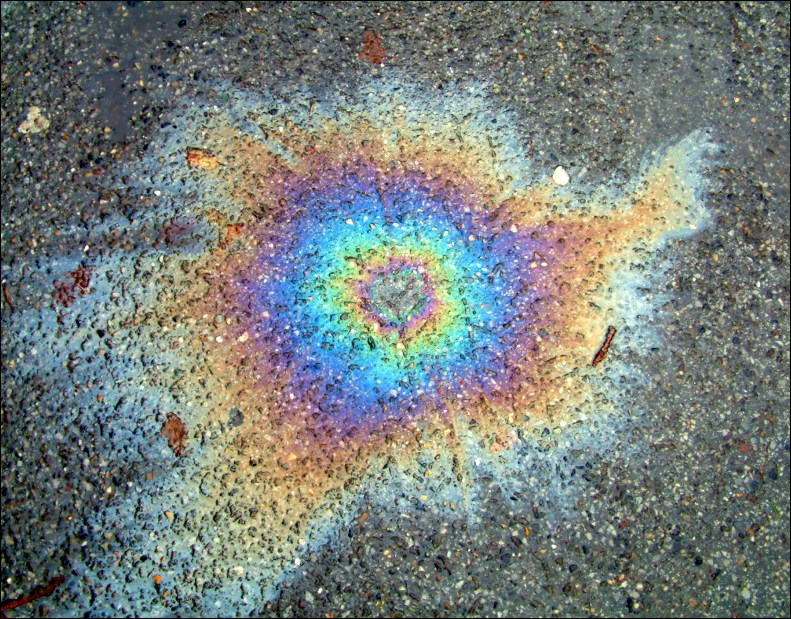
\includegraphics[width=0.6\textwidth]{images/2025-06-04-00-50-06.png}
 \caption{Plama benzyny na asfalcie}
 \end{figure}
\end{frame}

\begin{frame}{Bardzo prosty przykład II}
  \begin{figure}
 \centering
 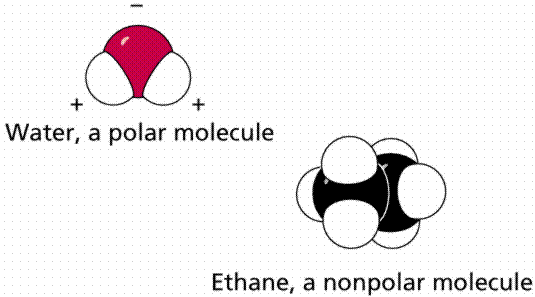
\includegraphics[width=0.6\textwidth]{images/2025-06-04-00-53-35.png}
 \caption{Cząstka wody vs. cząstka etanu}
 \end{figure}
\end{frame}

\begin{frame}{Energia swobodna}
  energia swobodna węglowodoru rozpuszczanego w wodzie: $$\mu_W = \mu_{W}^{\circ} + RT \ln X_W + RT \ln f_W$$

  energia swobodna węglowodoru rozpuszczanego w rozpuszczalniku: $$\mu_{HC} = \mu_{HC}^{\circ} + RT \ln X_{HC} + RT \ln f_{HC}$$

  węglowodory:
  $$\mu_{HC}^{\circ} - \mu_W^{\circ} = -2436 - 884n_C$$

  kwasy tłuszczowe:
  $$\mu_{HC}^{\circ} - \mu_W^{\circ} = 4260 - 825n_C$$
\end{frame}

\begin{frame}
  \begin{figure}
  \begin{subfigure}{0.45\textwidth}
 \centering
 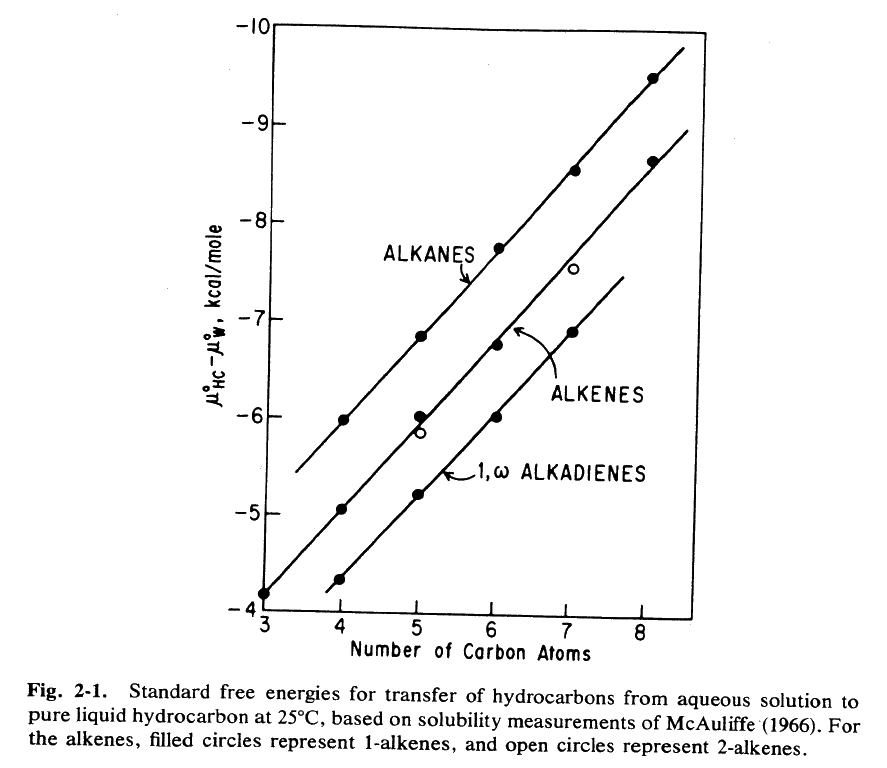
\includegraphics[width=0.9\textwidth, trim={3.5cm 2.5cm 3.5cm 0}, clip]{images/2025-06-03-22-57-41.png}
%  \caption{???????}
 \end{subfigure}
   \begin{subfigure}{0.45\textwidth}
 \centering
 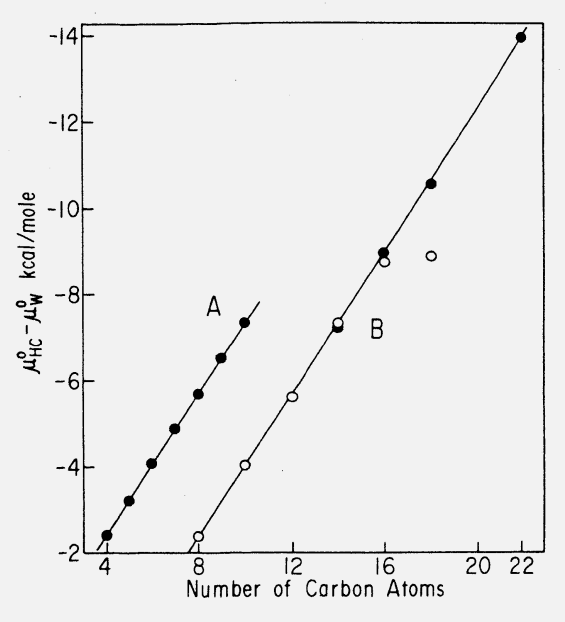
\includegraphics[width=0.9\textwidth]{images/2025-06-04-10-01-42.png}
%  \caption{}
 \end{subfigure}
 \caption{Zależność między energią swobodną a liczbą atomów węgla w cząsteczce węglowodoru (po lewej) i kwasu tłuszczowego (po prawej)}
  \end{figure}
\end{frame}

% \begin{frame}
  
% % kwasy tłuszczowe:
%   % $$\mu_{HC}^{\circ} - \mu_W^{\circ} = 4260 - 825n_C$$
%   % $$\mu_{HC}^{\circ} - \mu_W^{\circ} = -2436 - 884n_C$$



% \end{frame}

\section{Model sieciowy}

\begin{frame}{Struktura sieciowa wody}

  \begin{columns}
  \column{0.5\textwidth}
  \begin{figure}
 \centering
 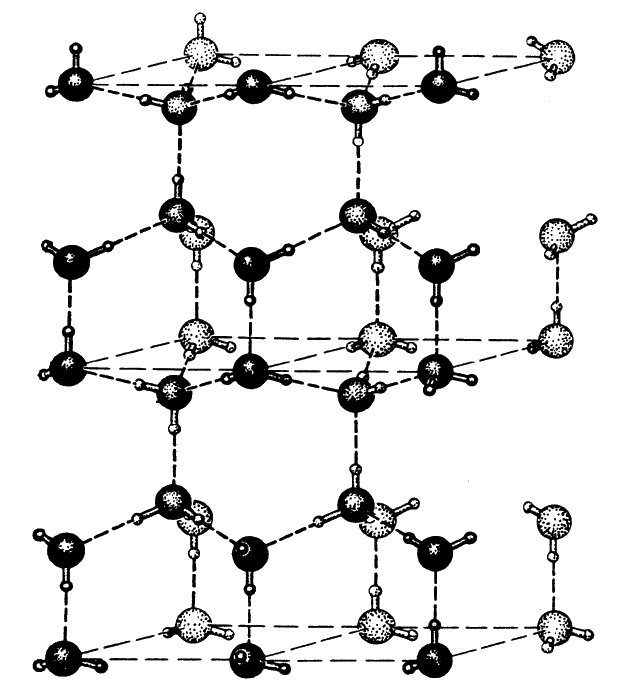
\includegraphics[width=0.7\textwidth]{images/2025-06-03-20-00-14.png}
 \caption{Struktura lodu I: duże kulki to atomy tlenu, mniejsze to atomy wodoru}
 \end{figure}
  \column{0.5\textwidth}
  \begin{figure}
 \centering
 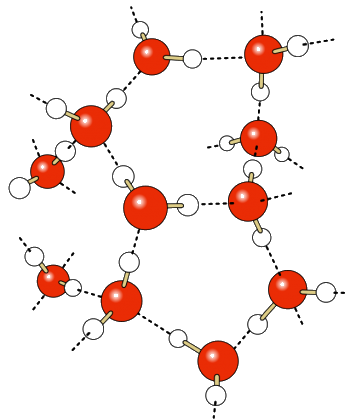
\includegraphics[width=0.7\textwidth]{images/2025-06-03-20-03-19.png}
 \caption{Wiązania wodorowe między cząsteczkami wody}
 \end{figure}
  \end{columns}
\end{frame}

\begin{frame}{Model Franka-Evansa}
\begin{columns}
\column{0.5\textwidth}
  \begin{figure}
 \centering
 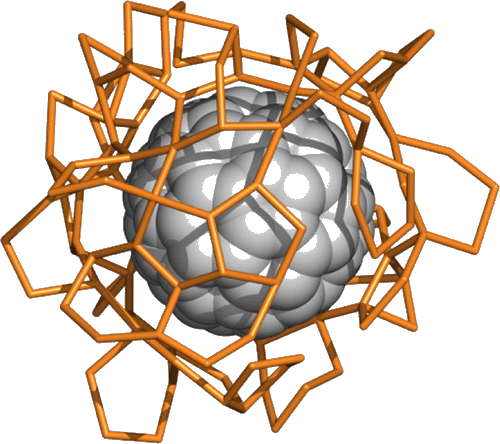
\includegraphics[width=0.9\textwidth]{images/2025-06-04-01-30-34.png}
 \caption{Struktura cząsteczek wody dookoła fulerenu w modelu Franka-Evansa (za: \cite{Grabowska_Kuffel_Zielkiewicz_2021})}
 \end{figure}
 \column{0.5\textwidth}
  % \begin{figure}
 \begin{figure}
 \centering
 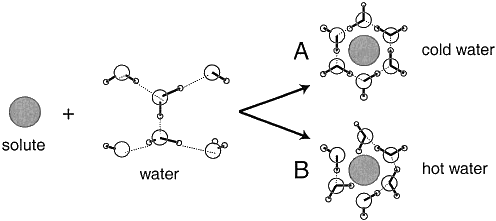
\includegraphics[width=0.9\textwidth]{images/2025-06-04-01-46-48.png}
 \caption{Ilustracja modelu Franka-Evansa w różnych temperaturach. \\W niskiej temperaturze cząsteczki wody przyjmują tylko kilka orientacji (niska entropia), aby uniknąć marnowania wiązań wodorowych. Większość konfiguracji wody jest w pełni związana wiązaniami wodorowymi (niska energia).\\ W gorącej wodzie więcej konfiguracji staje się dostępnych kosztem zrywania wiązań wodorowych. (za: \cite{Southall_Dill_Haymet_2002})}
 \end{figure}
\end{columns}
\end{frame}

\section{Micele}

\begin{frame}{Amfifile}
  \begin{figure}
 \centering
 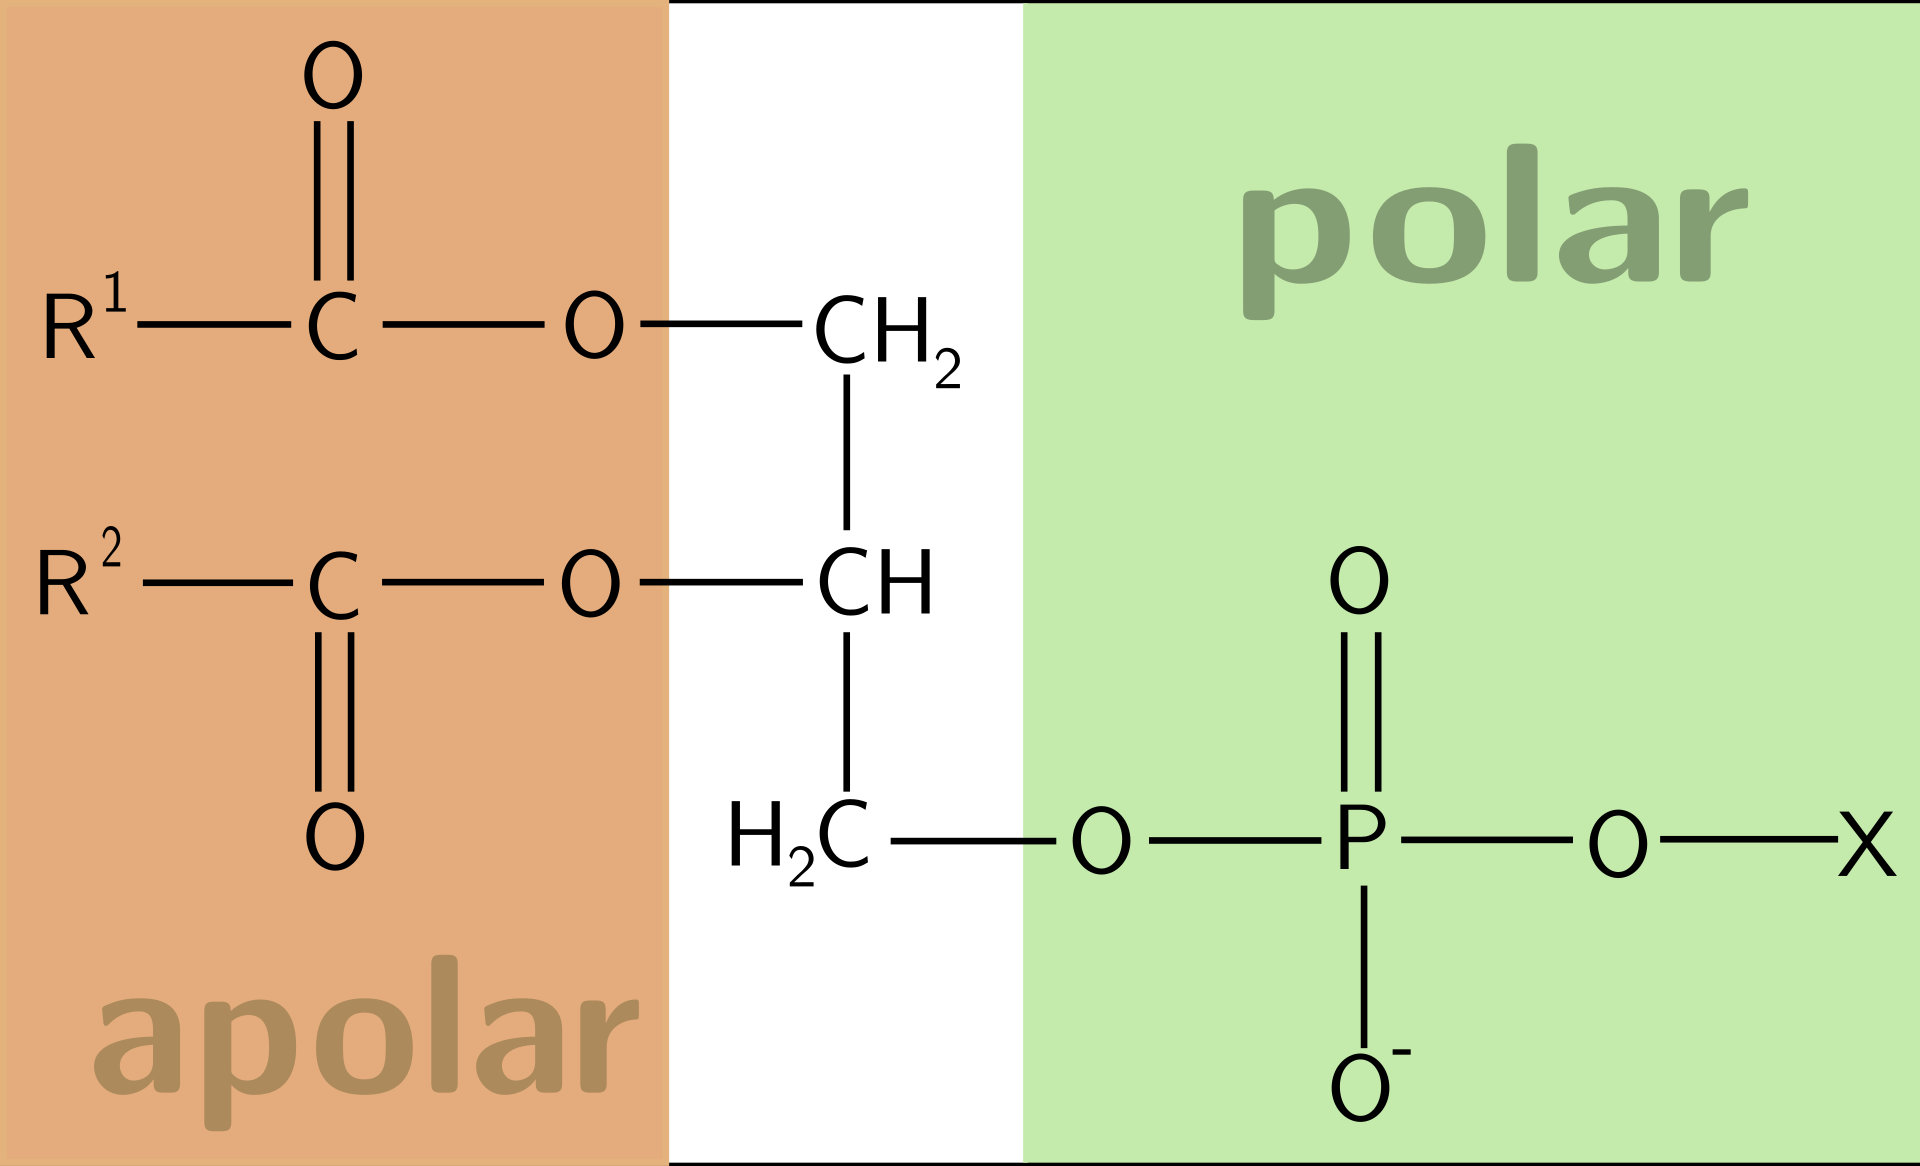
\includegraphics[width=0.5\textwidth]{images/2025-06-04-02-16-50.png}
 \caption{Glicerofosfolipid - przykład amfifilowej cząsteczki}
 \end{figure}
\end{frame}

\begin{frame}{Micele: definicja}{}
  \textbf{micele} -- agregowane produkty cząsteczek amfifilowych, które samoistnie tworzą się w roztworach wodnych
  \begin{columns}
  \column{0.5\textwidth}
  \begin{itemize}
  \item ogony: hydrofobowy rdzeń
  \item głowy: hydrofilowa powierzchnia
  \end{itemize}
  \column{0.5\textwidth}
\begin{figure}
 \centering
 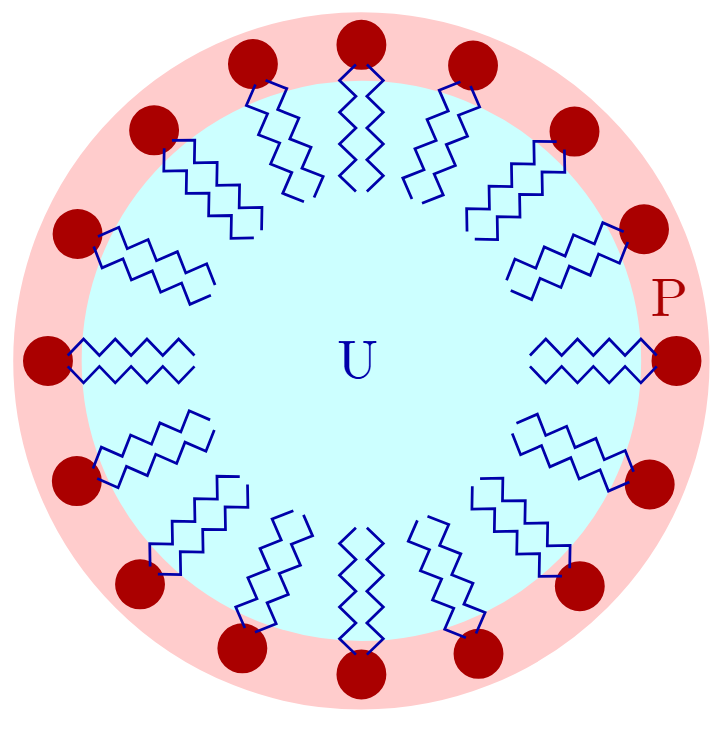
\includegraphics[width=0.5\textwidth]{images/2025-06-04-10-32-20.png}
 \caption{schemat miceli}
 \end{figure}
  \end{columns}
\end{frame}

\begin{frame}{Micele: termodynamika}
  $$\mu_{mic,m}=\mu_{mic,m}^\circ +\frac{RT}{m}\ln\frac{X_m}{m}$$
  \begin{itemize}
    \item $m$ -- liczba monomerów w miceli
    \item $X_m$ -- ułamek molowy monomerów w miceli
  \end{itemize}
\end{frame}

\begin{frame}{Micele: termodynamika I}

\begin{itemize}
  \item \textbf{CMC} (\emph{critical micelle concentration}) -- stężenie surfaktantu, powyżej którego spontanicznie tworzą się micele
  \item trochę jak \emph{przemiana fazowa} -- poniżej CMC mamy roztwór, powyżej CMC mamy micele
\end{itemize}

  \begin{figure}
 \centering
 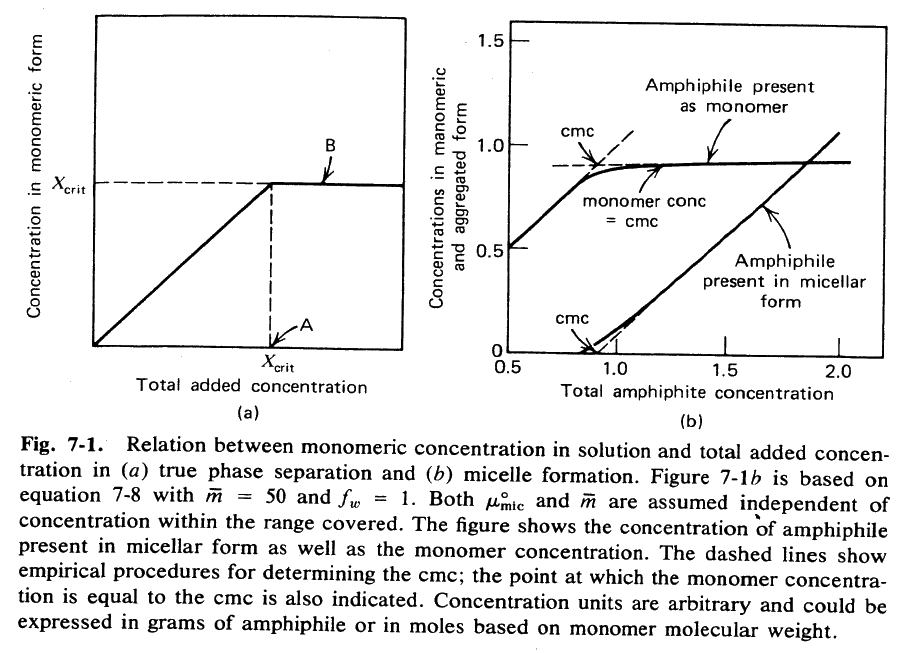
\includegraphics[width=0.65\textwidth, trim={0 5.8cm 0 0}, clip]{images/2025-06-04-02-08-15.png}
 \caption{Zależność między stężeniem monomerycznym w roztworze a całkowitym dodanym stężeniem w (a) rzeczywistym rozdziale faz i (b) tworzeniu miceli}
 \end{figure}
\end{frame}

\begin{frame}{Micele: termodynamika II}
\begin{figure}
 \centering
 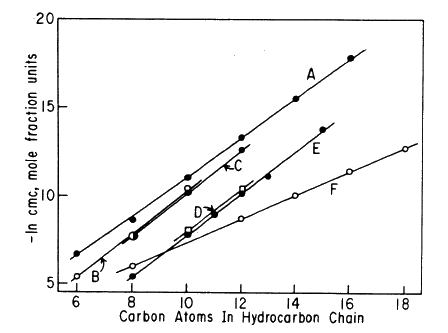
\includegraphics[width=0.5\textwidth]{images/2025-06-04-03-35-53.png}
 \caption{Zależność $(-\ln{} cmc)$ od liczby atomów węgla w łańcuchu węglowodorowym}
 \end{figure}

  
\end{frame}

\begin{frame}{Micele: kształt}
\begin{columns}
  \column{0.5\textwidth}
  parametr upakowania: $$P=\frac{v}{al}$$
  \begin{itemize}
    \item $v$ -- objętość ogona hydrofobowego
    \item $a$ -- powierzchnia równowagowa głowy hydrofilowej
    \item $l$ -- długość ogona hydrofobowego
  \end{itemize}
  \column{0.5\textwidth}
  \begin{figure}
 \centering
 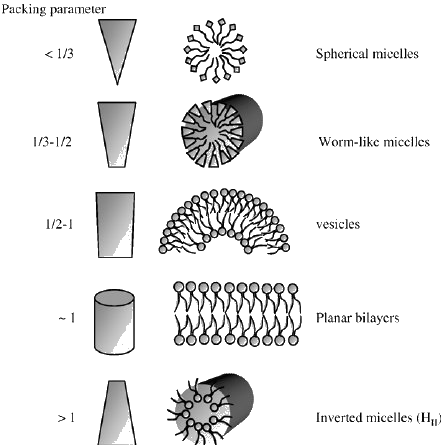
\includegraphics[width=0.9\textwidth]{images/2025-06-04-02-56-14.png}
%  \caption{}
 \end{figure}
\end{columns}
\end{frame}

% \begin{frame}{Micele: kształt II}
%   \begin{figure}
%  \centering
%  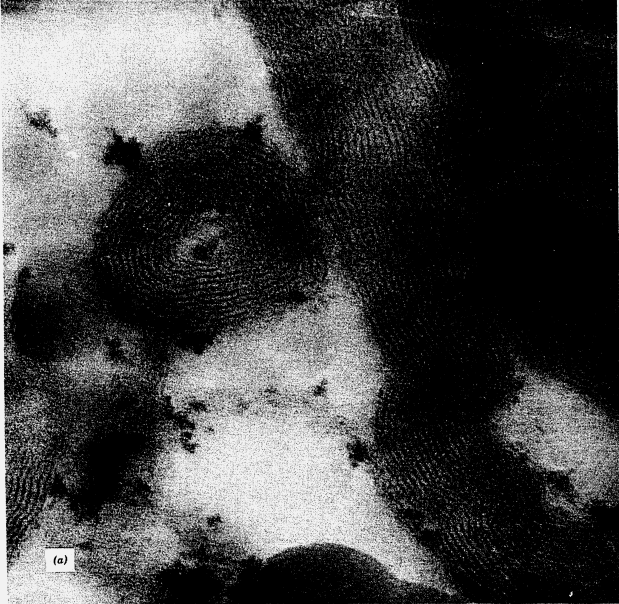
\includegraphics[width=0.5\textwidth]{images/2025-06-04-09-50-07.png}
%  \caption{}
%  \end{figure}
% \begin{figure}
%  \centering
%  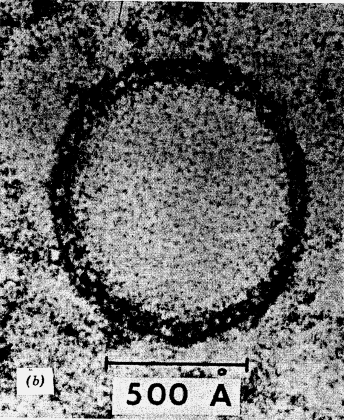
\includegraphics[width=0.5\textwidth]{images/2025-06-04-09-48-34.png}
%  \caption{}
%  \end{figure}
% \end{frame}

\section{Błony biologiczne}

% \begin{frame}{Błony biologiczne}{}

  
% \end{frame}

\begin{frame}{Mitochondria: przykład błony białkowo-lipidowej}
  \begin{figure}
\begin{columns}
    \column{0.5\textwidth}
 \centering
 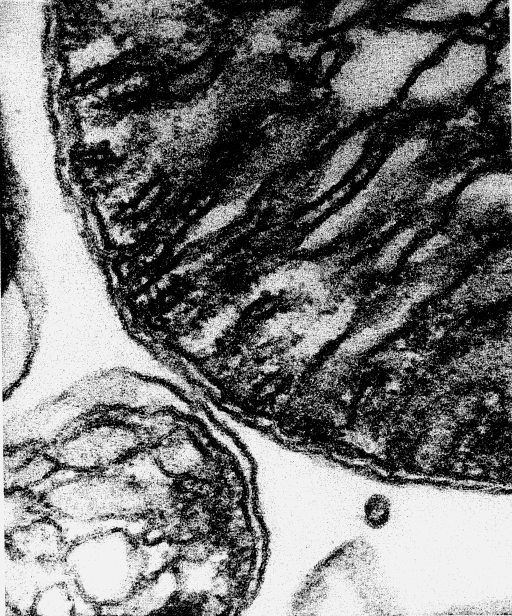
\includegraphics[width=0.8\textwidth]{images/2025-06-04-08-34-20.png}
 \column{0.5\textwidth}
 \caption{Zdjęcie z mikroskopu elektronowego przekroju mitochondrium. Widoczne są dwie błony: wewnętrzna i zewnętrzna. Wewnątrz mitochondrium znajduje się macierz mitochondrialna, a między błonami znajduje się przestrzeń międzybłonowa.}
\end{columns}
 \end{figure}
\end{frame}

\begin{frame}{Wykresy eksperymentalne}{}
\begin{figure}
\begin{subfigure}{0.3\textwidth}
 \centering
 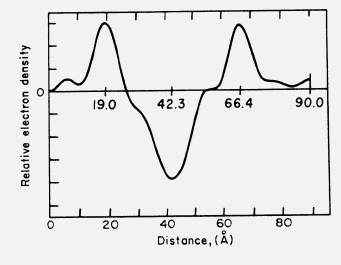
\includegraphics[width=0.9\textwidth]{images/2025-06-04-09-25-13.png}
 \caption{osłonka mielinowa królika}
 \end{subfigure}
 \begin{subfigure}{0.3\textwidth}
 \centering
 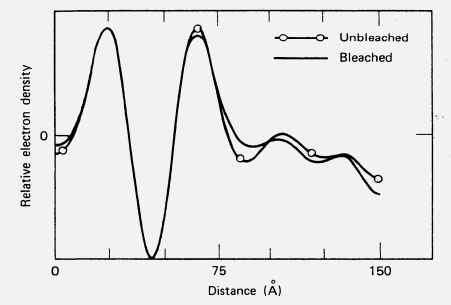
\includegraphics[width=0.9\textwidth]{images/2025-06-04-09-25-39.png}
 \caption{błony pręcika siatkówki}
 \end{subfigure}
 \begin{subfigure}{0.3\textwidth}
 \centering
 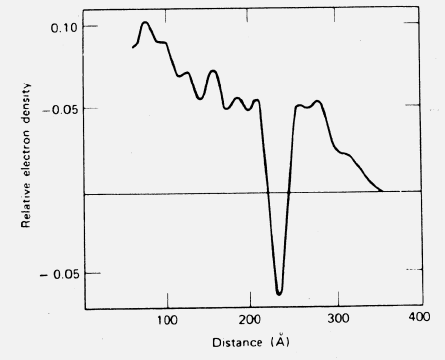
\includegraphics[width=0.9\textwidth]{images/2025-06-04-09-26-09.png}
 \caption{wirus \emph{A. sindbis} (średnia radialna)}
 \end{subfigure}
  \caption{Zależność gęstości elektronowej błon biologicznych od odległości}
\end{figure}
\end{frame}

\begin{frame}
  \begin{figure}
 \centering
 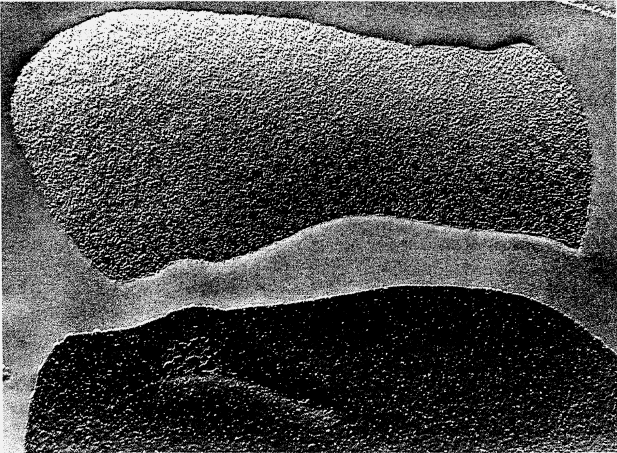
\includegraphics[width=0.7\textwidth]{images/2025-06-04-07-34-44.png}
 \caption{\emph{Freeze fracture electron microscopy} błony erytrocytu (na górze: wewnętrze komórki, na dole: zewnętrzna powierzchnia błony)}
 \end{figure}
\end{frame}

\section*{}


\begin{frame}{Bibliografia}{}
  \nocite{*}
  \printbibliography[heading=none]
\end{frame}

\transblindshorizontal

\begin{frame}{~}{}
  \transglitter
  \vspace{-1cm}
\begin{figure}
\centering
  \begin{tikzpicture}
    \duck[parrot, body=gray!30!yellow, head=gray!30!yellow, bill=red, torch=gray!70!brown, tshirt=blue!40!black, ribbon=gray, bowtie=blue!50!white, crazyhair=black]
    %\addwater{blue!50!cyan}
    \fill[cyan!20!white] (-1.4,1.8) ellipse (1.8 and 0.5);
\fill[cyan!20!white] (-0.2,1.54) -- (0.2,1.35) -- (0.0,1.6) -- cycle;
\node at (-1.4,1.8) {dziękuję za uwagę};
  \end{tikzpicture}
  \end{figure}


  
  \begin{figure}
  \centering
        % 
\includegraphics[height=0.3\linewidth]{images/2025-05-13-15-25-41.png}\\
      \qrcode[height=0.3\textwidth]{https://github.com/falcotinnunculus/przezrocza/blob/wladca/sb22/hydro.pdf}
  {\scriptsize \url{https://github.com/falcotinnunculus/przezrocza/blob/wladca/sb22/hydro.pdf}}

  \end{figure}
% \vspace{-5.3cm}
% \transparent{0.7}
  % \begin{figure}
      % \centering
      % \caption{Caption}
      % \label{fig:enter-label}
  % \end{figure}
\end{frame}


\end{document}